\chapter{Stability \& Control}
\setlength{\parindent}{15pt}
\label{ch:stab_cont}

The stability and control design and analysis will be explained and presented in this chapter. First of all, \autoref{sec:desi_appr_snc} will clarify the approach followed in order to design and analyse the UAV for stability and control. Secondly, the assumptions used for the analysis are stated in \autoref{sec:assu_snc}. Next, \autoref{sec:anal_snc} explains the methods used to design and analyse the UAV and presents the results of the design and analysis. Finally, the verification and validation of the analysis models, the tools used, and the results are presented in \autoref{sec:veri_vali_snc}.

\section{Design Approach}
\label{sec:desi_appr_snc}

\autoref{fig:StabContFlow} shows the work flow diagram for the stability and control design process. Here, the blue square indicates the design phase for longitudinal stability, the green square indicates the design phase for lateral and directional stability, and the yellow square indicates the design phase comprising the manoeuvres in transition, horizontal, and vertical flight. Different design options can be considered in order to control the UAV and to ensure stability. In the concept selection phase, the decision has been made to have a tail for stability and control surfaces for control in horizontal flight, whereas propellers are used for control and stability in vertical flight. First of all, the tail was sized for longitudinal and lateral control and stability considering the critical case of one engine failure. A tail configuration was selected based on effectiveness and controllability. The required surface area of the vertical and horizontal tail were calculated and the optimal incidence angle of the horizontal tail was found. Simultaneously, the c.g. range needed to be estimated and controlled using the position of the wing as a balancing tool. Secondly, the control surfaces and actuators were sized in order to provide the required angular acceleration in horizontal flight. Thereafter, the propeller power split in order to perform manoeuvres during vertical flight was calculated. Finally, the transition phase was considered and a series of actions was defined in order to have a smooth transition.  %this is an overview of the work flow

The design process of the tail is an iterative process where the global c.g. position and the position of the leading edge of the wing change throughout the design. In order to know the global c.g. the tail needs to be sized. Vice versa, in order to size the tail, the c.g. needs to be known. By using the mass budget and an initial placement of the subsystems, an initial c.g. estimation was made. This estimation was used as a starting point for the tail sizing and wing positioning. Eventually, a more updated c.g. was found using CATIA, so the design could be iterated. Likewise, in order to calculate the position of the leading edge, an initial position needs to be assumed. This leading edge position is needed to calculate the control and stability curves. When the control and stability curves are combined with the c.g.range curves, a new optimal leading edge position can be found. This new leading edge position has to be iterated into the control and stability curves.  %this is some more explanation on the tail iteration

Also the design process of the control principle is an iterative process. Similar to the c.g., the Moment Of Inertia (MOI) changes throughout the design phase. Again, an initial estimation of the MOI was made in order to estimate the required control moments. Next, in order to size the control surfaces, the arm needs to be known which depends on the size of the control surface. Therefore, another iteration process was needed. %here will be some more explanation on the control surface iteration

\nomenclature[A]{MOI}{Moment of Inertia}

\begin{figure}[htb]
    \centering
    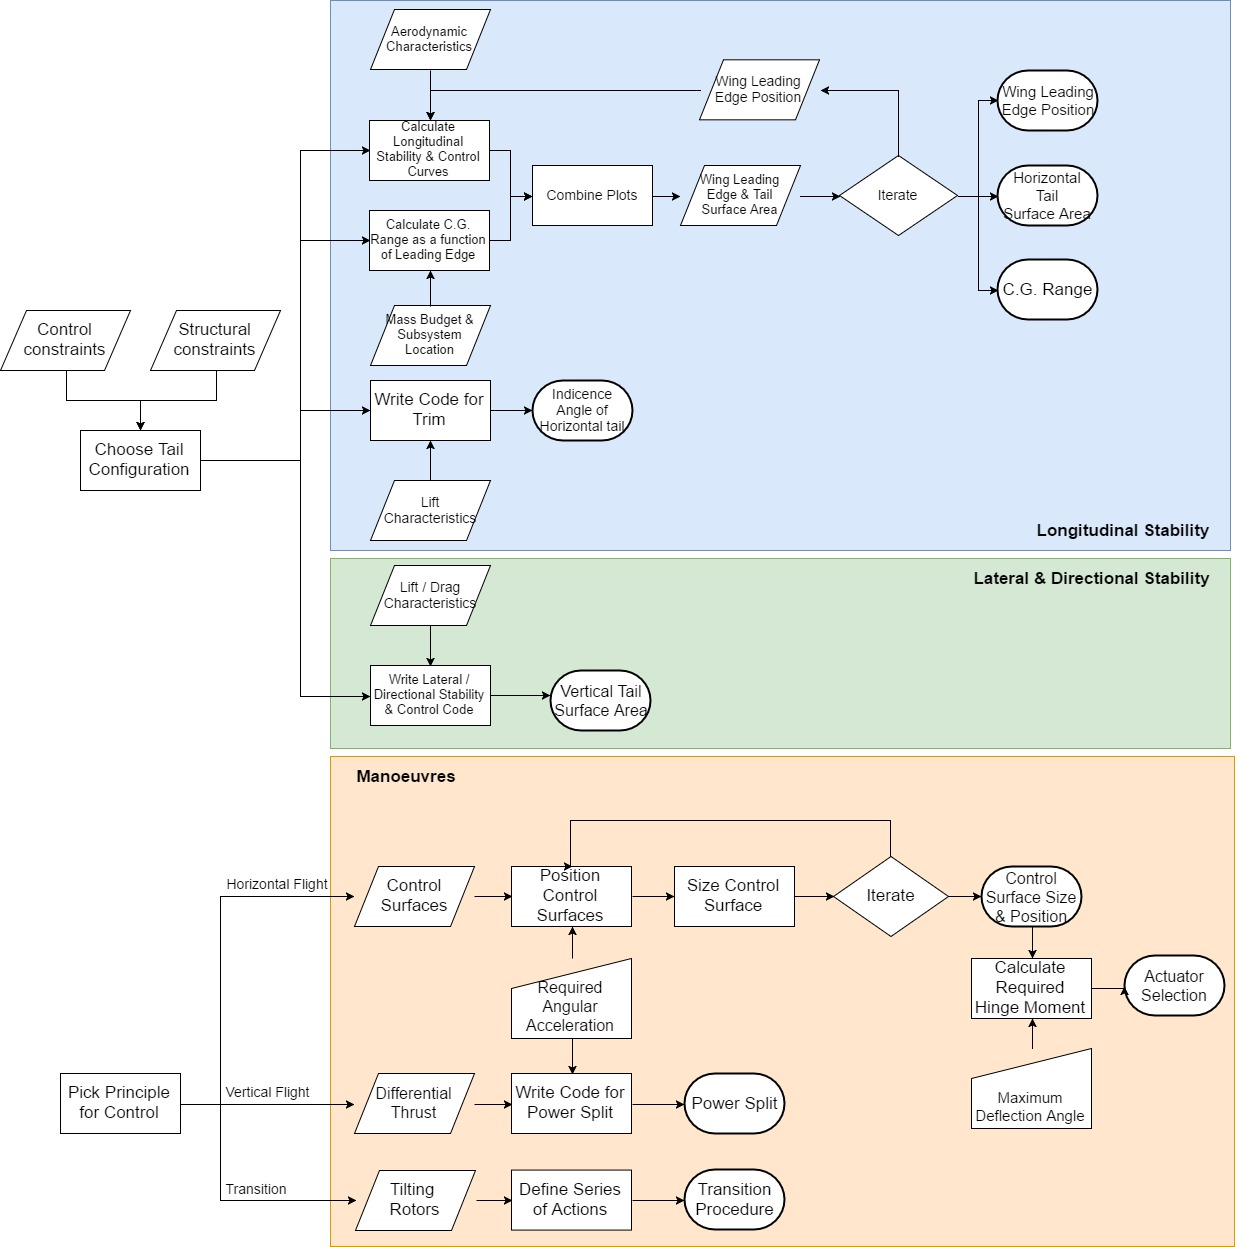
\includegraphics[width=\textwidth]{StabilityandControl/Figures/workflowSNC}
    \caption{Work Flow Diagram for the Stability \& Control Design Process}
    \label{fig:StabContFlow}
\end{figure}

\section{Assumptions}
\label{sec:assu_snc}

\begin{itemize}
    \item It is assumed that the c.g. of the UAV coincides with the a.c. of the wing. With the actual c.g. range located between 0.55 m and 0.74 m from the nose, and the a.c. of the wing located at 0.60 m from the nose, the maximum distance between them is 0.14 m. Therefore, this assumption can be used in the design process without heavily affecting the final results.
    \item It is assumed that the lift coefficient of the horizontal tail during stall, with elevator fully deflected, is equal to -0.8. This value is derived from statistical data for aircraft with adjustable tails \cite{SEAD}.
    \item It is assumed that the resultant force of a control surface goes through half the chord of the control surface. Conventionally, the resulting force is taken through a quarter chord. However, the flow over the control surface is heavily affected by the airfoil in front of it. By assuming the resultant force goes through half the chord, the arm of the force to the hinge is slightly larger than the actual arm. Therefore, the actuators will be slightly over-designed.
    %\item The C$_{m_{ac}}$ of the fuselage and engine nacelles are assumed to be negligible compared to the C$_{m_{ac}}$ of the wing. This assumption is erased because we do include the fuselage contribution
    \item It can be assumed that the downwash at the horizontal tail-plane is negligible. Based on statistical relations based on the horizontal and vertical distance between the wing and tail, the downwash at the tail will have a magnitude of 10$^{-3}$. Hence, this assumption can be considered valid. 
    \item It can be assumed that the tail/wing speed ratio, $\frac{V_h}{V}$, is equal to one. This is a valid assumption since a T-tail is used with sufficient distance between the tail and the vortex shed of the wing. Hence, the perturbations in the flow at the tail caused by the fuselage are negligible. 
    \item It is assumed that the UAV has a plane of symmetry across in the x,y-plane. Hence, the c.g. can be assumed to lie on the plane of symmetry. This assumption can be considered valid since the layout of the plane is symmetrical. Some small deviations may exist because of a non-symmetrical placing of internal components or non-symmetrical payload bay mass distribution.
    \item It is assumed that the fuselage doesn't generate lift. From the CFD analysis done by the aerodynamic department, the fuselage lift coefficient has an order of magnitude of 10$^{-3}$. Therefore, this assumption can be used without affecting the results.
    \item The centre of gravity of the payload bay is assumed to lie between the 10 cm and 50 cm mark measured from the front of the payload bay. This takes into account two loading categories: 1. the need to carry batteries and at the same time having sufficient continuous space for useful payload; 2. the need to carry heavy payloads (i.e. 10 kg) which occupy the entire payload bay. The mass of heavy payloads which occupy the entire payload bay is assumed to be distributed homogeneously throughout the payload volume.
    \item Whilst sizing the vertical tailplane it is assumed that the aerodynamic force induced as a result of side-slip acts perpendicular to the moment arm from the centre of gravity. In reality, the perpendicular component of this aerodynamic force is slightly smaller (scaled with the cosine of the side-slip angle) resulting in a slightly smaller required surface. This assumption therefore makes the calculated surface slightly conservative.
    \item Conservation of momentum and energy laws are assumed to provide sufficient accuracy when calculating the power required during the vertical flight phase. In reality, the motor and propeller efficiency must also be considered. The use of conservative inputs (namely a higher power required to hover) offsets whatever insufficiency the conservation of momentum and energy laws might introduce.
    \item The torque delivered by the motors is assumed to be proportional to the current delivered. It is also assumed that the angular velocity of the motors is proportional to the voltage applied. In reality this is loosely accurate, however, it not entirely correct to assume both torque and angular velocity vary linearly. This does not affect the required power splits, however, the motor-propeller combination must be tested experimentally to see how the output power varies with varying current and voltage.
\end{itemize}

\section{Analysis}
\label{sec:anal_snc}
This section shows the methods used to analyse and design the UAV for stability and control, and presents the final results. 

\subsection{Tail Configuration}
First of all, a tail configuration was picked based on the effectiveness, structural weight, and controllability of the tail-planes. Since downwash caused by the vortex of the wing reduces the effectiveness of the tail, a horizontal tailplane located outside of the downwash is preferred. Furthermore, it would be favourable to have tailplanes where roll and yaw, and longitudinal and lateral control are separated from each other. The structural weight of the tail was also taken into account when choosing a tail configuration. For example, a V-tail has a reduced amount of components. 
A T-tail was chosen as the final tail configuration mainly because downwash can be completely neglected and the control surfaces can be completely separated. At the same time, the structural weight can stay within the budget.

\begin{equation}
\label{eq:trimbla}
    C_{L_{h}} = C_{L_{cruise}}\frac{S}{S_h}\frac{(x_{c.g.}-x_{a.c._{w}})}{(x_{a.c._{h}}-x_{c.g.})}
\end{equation}

Next, the incidence angle of the horizontal tailplane was calculated in order to be trimmed without the need of deflecting the elevator. The required tail lift coefficient was calculated for cruise conditions using \autoref{eq:trimbla} which is derived from the trim equation. The optimal incidence angle can be found by finding the corresponding angle of attack in the $C_L$-$\alpha$ curve of the tail.

\subsection{Longitudinal Stability \& Control}
The UAV is required to be longitudinally statically stable. This means that it is able to react to a change in the angle of attack by generating an opposite pitching moment to restore the former state of equilibrium. In order to achieve stability, the c.g. should be positioned in front of the neutral point. The position of the neutral point is dependent on the ratio of wing/tail surface areas. When taking into account a Safety Margin (SM) of 0.05\footnote{AE3211-I Lecture 5 - Requirement Analysis and Design principles for A/C stability \& control (Part 1)}, the maximum position of the c.g. (in order to be stable) can be calculated as a function of the wing/tail surface ratio, as can be seen in \autoref{eq:stabSM}. In this equation, a macron (the bar on top of a symbol) indicates it is divided by the mean aerodynamic chord of the wing. The downwash is assumed to be zero and wing/tail speed ratio can be assumed to be equal to one since a T-tail configuration is used. The distance between the wing and tail, $l_h$, can be estimated by assuming an initial position of the leading edge of the wing and iterating it. The other parameters are aerodynamic characteristics.

\begin{equation}
\label{eq:stabSM}
    \bar{x}_{c.g._{max}}=\bar{x}_{a.c.}+\frac{C_{L_{\alpha_h}}}{C_{L_{\alpha_{A-h}}}}\Big(1-\frac{d\epsilon}{d\alpha}\Big)\frac{S_h l_h}{S\bar{c}}\Big(\frac{V_h}{V}\Big)^2-SM
\end{equation}

\nomenclature[B]{$x_{c.g._{max}}$}{Maximum centre of gravity position from the nose \nomunit{m}}
\nomenclature[B]{$x_{c.g._{min}}$}{Minimum centre of gravity position from the nose \nomunit{m}}
\nomenclature[B]{$x_{a.c.}$}{Position of the aerodynamic centre of the wing from the nose \nomunit{m}}
\nomenclature[B]{$C_{L_{\alpha_h}}$}{Lift slope coefficient of the tail \nomunit{-}}
\nomenclature[B]{$C_{L_{\alpha_{A-h}}}$}{Lift slope coefficient of the aircraft minus tail \nomunit{-}}
\nomenclature[B]{$\frac{d\epsilon}{d\alpha}$}{Downwash \nomunit{-}}
\nomenclature[B]{$S$}{Wing surface area \nomunit{m$^2$}}
\nomenclature[B]{$S_h$}{Tail surface area \nomunit{m$^2$}}
\nomenclature[B]{$l_h$}{Distance between the a.c. of the wing and the a.c. of the tail \nomunit{m}}
\nomenclature[B]{$\bar{c}_w$}{Mean aerodynamic chord of the wing \nomunit{m}}
\nomenclature[B]{$\frac{V_h}{V}$}{Tail/wing speed ratio \nomunit{-}}
\nomenclature[A]{SM}{Safety Margin}

Additionally, the UAV is required to be controllable. An aircraft is said to be controllable when it is able to be trimmed for a certain aircraft configuration. In other words, a combination of wing and tail lift coefficient should result in a zero total aircraft moment coefficient. In order to achieve controllability, the c.g. has to be positioned behind a certain limit point. This point can be found as a function of the wing/tail surface area by using the trim equation. Here the moment generated by the wing around the c.g. has to be equal to the moment generated by the tail around the c.g.. When rewriting this equation, the minimum position of the c.g. (in order to be controllable) can be calculated as a function of the wing/tail surface area, as can be seen in \autoref{eq:stabeq}. Again, the wing/tail speed ratio can be assumed to be equal to one. The distance between the wing and tail can be estimated and iterated. The aerodynamic characteristics are input in the remaining parameters.

\begin{equation}
\label{eq:stabeq}
    \bar{x}_{c.g._{min}}=\bar{x}_{a.c.}-\frac{C_{m_{a.c.}}}{C_{L_{A-h}}}+\frac{C_{L_{h}}}{C_{L_{A-h}}}\frac{S_h l_h}{S \bar{c}}\Big(\frac{V_h}{V}\Big)^2
\end{equation}

These two equations can be plotted with the c.g. measured from the leading edge divided by the mean aerodynamic chord on the x-axis, and the wing/tail surface area on the y-axis. This plot is called the scissor plot, presented as the blue curves in \autoref{fig:scissor}. In between the two curves lies the region where, if the c.g. is positioned there, the aircraft is stable and controllable. The position of the wing is used as a balancing tool in order to get the actual c.g. range shifted to the optimal position in order to have the lowest wing/tail ratio. Visually, this means that a plot of the c.g. range as a function of the leading edge has to be combined and shifted vertically to the scissor plot until the range of the c.g. plot matches with the width of the scissor plot.

\begin{figure}[htb]
    \centering
    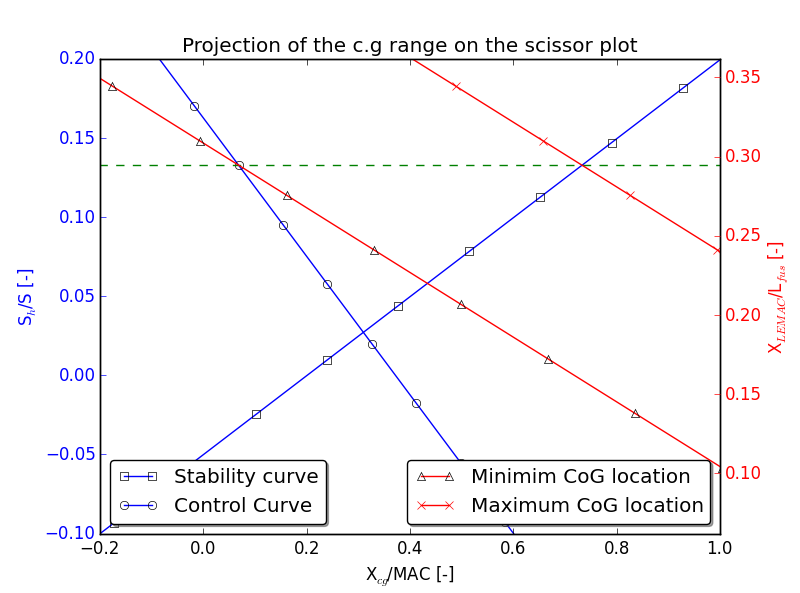
\includegraphics[width=0.7\textwidth]{StabilityandControl/Figures/Scissor}
    \caption{Projection of the C.G. Range on the Scissor Plot}
    \label{fig:scissor}
\end{figure}

\nomenclature[B]{$x_{LE}$}{Leading edge position of the wing from the nose}
\nomenclature[B]{$L_{fus}$}{Fuselage length}

Now the c.g. plot needs to be calculated. Here, the c.g. range is plotted with the c.g. measured from the leading edge divided by the mean aerodynamic chord on the x-axis, and the wing leading edge divided by the length of the fuselage on the y-axis. Hence, the x-axes of both the scissor and c.g. plots are the same. In order to calculate the c.g. range, \autoref{eq:c.g.r} is used. Here, $m_i$ is the mass of a subsystem, $x_i$ is the c.g. of the subsystem, and n is the number of subsystems. Since the c.g. of the payload bay has a minimum and a maximum value, a range of c.g. values is found. Furthermore, the c.g. value depends on the x-location of the wing, which depends on the position of the leading edge of the wing. Hence, the c.g. range can be expressed as a function of the wing leading edge over the length of the fuselage. The curves for the maximum and minimum c.g. ranges are presented as the red curves in \autoref{fig:scissor}.

\begin{equation}
\label{eq:c.g.r}
    x_{c.g.} = \frac{\sum_{i=1}^{n} {x_i\cdot m_i}}{\sum_{i=1}^{n_i} {m_i}}
\end{equation}

By shifting the c.g. plot over the scissor plot, one can see in \autoref{fig:scissor} that an optimal value for the wing/tail ratio, and leading edge over fuselage length ratio can be found. This is indicated by the green dotted line extended between both y-axes. The final results are presented in \autoref{tab:scissorres}. The final values used to calculate the total c.g. position can be found in \autoref{tab:cgbreakdown}.

\begin{table}[htb]
\centering
\caption{Results of the Scissor and c.g. Plot}
\label{tab:scissorres}
\begin{tabular}{lll}
\toprule
\textbf{Parameter} & \textbf{Value} & \textbf{Unit} \\ \midrule
$x_{cg_{min}}$     & 0.55           & m             \\ \hdashline
$x_{cg_{max}}$     & 0.74           & m             \\ \hdashline
$x_{LE}$           & 0.53           & m             \\ \hdashline
$S_h$              & 0.106          & m$^2$      \\  \bottomrule
\end{tabular}
\end{table}

\subsection{Lateral/Directional Stability \& Control}

In this section, the lateral and directional stability and control of the UAV is analysed. In order to achieve this, the vertical tail area of the system has to be designed. Using wing mounted engines, the critical design case for vertical tail sizing is obtained in the one-engine-out condition. In this case, the remaining engine creates a yaw-moment which needs to be counteracted using the vertical tailplane. Although a rudder deflection might also be used for this, the moment should only be based on the vertical tailplane, as directional yaw control of the aircraft in both directions is still needed and achieved using rudder deflections.

First, a necessary yaw angle at which equilibrium is achieved needs to be defined. It was assumed, that in one engine out condition, equilibrium will be obtained at a yaw angle of 5$^\circ$. Then, the UAV velocity will be reduced to maximum range speed, $V_{range} = 27 \frac{m}{s}$, in order to be able to fly to the best landing location. In case the engine fails at a lower velocity, the drag will be lower and in turn less thrust is required. This will reduce the yaw moment and thus flying at lower velocities will also be possible. Using aerodynamic properties, the thrust required for the remaining engine is now obtained with \autoref{eq:drag_vertical}. 

\begin{equation}
    T = C_D\cdot\frac{1}{2}\cdot\rho\cdot V^2_{range}\cdot S
    \label{eq:drag_vertical}
\end{equation}

Then, considering the fact that the engines are all mounted at the same distance $y_{engine}$ from the centre of gravity, the yaw moment created by the one-engine-out condition is obtained using $M = T\cdot y_{engine}$. This yaw moment has to be counteracted by the vertical tailplane at an angle of side-slip of $\beta = 5^\circ$. As the moment arm, airfoil, velocity, and the sweep angle of the vertical tailplane are known, the required surface area can be calculated using \autoref{eq:surf_area_vert}.

\nomenclature[B]{$y_{engine}$}{Distance between engines and centre of gravity along the wingspan \nomunit{m}}

\begin{equation}
    S_{vertical} = \frac{2\cdot M_{yaw}}{l_v\cdot C_{L_{\beta_v}}\cdot \beta\cdot\rho\cdot (V_{range}\cdot cos(\lambda_{v}))^2}
    \label{eq:surf_area_vert}
\end{equation}

In \autoref{eq:surf_area_vert}, $M_{yaw}$ is the yaw moment generated by the engine, $l_v$ the distance between the centre of gravity and the aerodynamic centre of the vertical tailplane, $\lambda_v$ the sweep angle of the vertical tailplane, and $C_{L_{\beta_v}}$ the lift coefficient/sweep angle slope obtained using an XFLR5 analysis. For lateral stability, the vertical tail must have a surface area of 0.026 $m^2$.
\nomenclature[B]{$M_{yaw}$}{Yaw moment \nomunit{Nm}}
\nomenclature[B]{$l_v$}{Distance between centre of gravity of the UAV and the aerodynamic centre \nomunit{m}}
\nomenclature[G]{$\lambda_v$}{Sweep angle of the vertical tailplane \nomunit{rad}}
\nomenclature[B]{$C_{L_{\beta_v}}$}{Vertical tailplane lift coefficient slope \nomunit{-}}




%Creates roll moment --> counteracted using ailerons 



\subsection{Control Surfaces}

In this section the size and position of the control surfaces are determined. These are ailerons for roll control, an elevator for pitch control, and a rudder for yaw control. Then, the hinge moment is calculated in order to select suitable servos. 

The design of the control surfaces is dependent on the angular accelerations required. From requirements SUB-W-7.3, SUB-T-2.2, and SUB-T-2.3, the following angular accelerations are defined.

\begin{equation*}
    \alpha_{roll} = \alpha_{pitch} = 45 \frac{^\circ}{s^2} \quad \alpha_{yaw} = 6 \frac{^\circ}{s^2}
\end{equation*}

\nomenclature[G]{$\alpha_{roll}$}{Angular roll acceleration \nomunit{rad/s$^2$}}
\nomenclature[G]{$\alpha_{pitch}$}{Angular pitching acceleration \nomunit{rad/s$^2$}}
\nomenclature[G]{$\alpha_{yaw}$}{Angular yaw acceleration \nomunit{rad/s$^2$}}

Using the moments of inertia, the torque required is obtained using \autoref{eq:newton2}. These torques have to be created by the control surfaces and hence depend strongly on the physical location of the control surfaces. The elevator is located at the trailing edge of the horizontal tailplane. The ailerons are positioned as far away from the fuselage as possible in order to maximise the moment arm. In order to avoid twisting the control surfaces themselves, they can not be positioned at the wing tips. Therefore, they will be positioned just before the start of the wing twist. The rudder is located at the trailing edge of the vertical tailplane. The locations of the control surfaces lead to the moment arms.

\begin{equation}
    T = I \cdot \alpha
    \label{eq:newton2}
\end{equation}

With the moment arms and the torque required, one can calculate the required force for the surface. The force generated by deflecting the surfaces to an angle of $\delta$ is given by \autoref{eq:cont_forc}.

\begin{equation}
    F = C_{n_{\delta}}\cdot \delta\cdot\frac{1}{2}\cdot\rho\cdot V^2 \cdot S
    \label{eq:cont_forc}
\end{equation}

In \autoref{eq:cont_forc}, $C_{n_{\delta}}$ is obtained using an XFLR5 analysis. In order to size the control surfaces, stall speed is assumed. This ensures that the surface is capable of providing enough force for the whole speed range. Comparing control surface deflection angles of different aircraft, the following maximum deflection angles were defined: 

\nomenclature[B]{$C_{n_{\delta}}$}{Normal force gradient \nomunit{-}}
\nomenclature[G]{$\delta$}{Control surface deflection angle \nomunit{deg}}
\begin{equation*}
    \delta_{elevator_{max}} = 28^\circ\quad\delta_{rudder_{max}} = 25^\circ\quad\delta_{aileron_{max}} = 30 ^\circ
\end{equation*}

Using these parameters, it is now possible to calculate the surface area of the different control surfaces by rearranging \autoref{eq:cont_forc}. 
Now, the aileron chord is assumed to be 20\% of the wing chord, elevator span to be 70\% of the horizontal tailplane span, and rudder span to be 90\% of the vertical tailplane span. This makes it possible to calculate the different dimensions for the surface area. 

Using the dimensions of the different control surfaces, an appropriate servo has to be chosen. For this, it is necessary to calculate the torque required to maintain a the maximum certain deflection. 

\begin{figure}[htb]
    \centering
    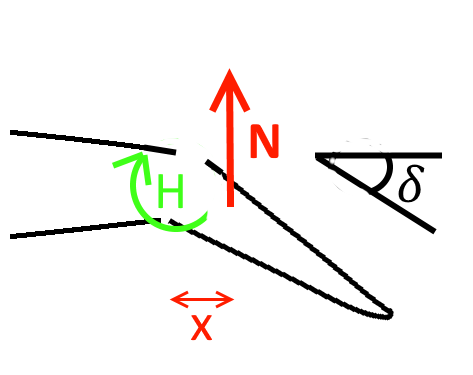
\includegraphics[scale=1]{./StabilityandControl/Figures/hinge}
    \caption{Hinge Moment Created by the Control Surface Force}
    \label{fig:hing}
\end{figure}

As can be seen in \autoref{fig:hing}, the hinge moment created by the normal force N is dependant on the aerodynamic centre of the control surface. For calculation purposes it is assumed that the force acts halfway through the chord. The actual hinge moment will be lower as the aerodynamic centre is in general located at the quarter-point of the chord. Then for the sizing, worst case scenario is assumed, meaning flying at maximum speed of 200 $\frac{km}{s}$ and deflecting the control surface to maximum deflection. The control force is then calculated using \autoref{eq:cont_forc}, which, multiplied by the moment arm, gives the hinge moment. The final control surface results are illustrated in \autoref{tab:cont_surf}.

\nomenclature[B]{$N$}{Normal force \nomunit{N}}

\begin{table}[htb]
    \centering
    \caption{Control Surface Properties}
    \label{tab:cont_surf}
    \begin{tabular}{lcccc}
      \toprule
        & Span [cm]& Chord [cm]& Surface Area [$cm^2$] & Maximum Hinge Moment [Ncm] \\
      \midrule
      Aileron & 17.1 & 3.69 & 63.1 &23\\\hdashline
      Elevator & 47.2 &2.89& 136  &36\\\hdashline
      Rudder & 16.3 & 2.67 & 43.4 &12\\\bottomrule
    \end{tabular}
\end{table}

Four SAVÖX SC-0254MG servos are used for both ailerons, the elevator and the rudder. They are able to deliver a torque of 62 Ncm at minimum power consumption. \footnote{\url{https://www.hacker-motor-shop.com/Servos/Savoex-Servos/Servos-Flugmodelle/Servo-SAVOeX-SC-0254MG.htm?SessionId=&a=article&ProdNr=80101005&p=6264}, Accessed 22-06-2017}

\subsection{Vertical Flight Manoeuvres} %This is subject to change

During the vertical flight phase of the the UAV various manoeuvres have to be considered, namely pitch, roll and yaw, all of which are achieved purely through varying the thrust level of the four propellers. By varying the power applied to motor couples the required moments about the axis around which the manoeuvre takes place can be produced. In this section the power required to achieve specified angular accelerations about the three axes will be characterised. However it is necessary to first define the locations of the four motors with respect to the centre of gravity. It is important to note that the conventional body axis system with its origin located at the centre of gravity is used in this section; i.e. the $x$-axis points in the direction of the nose, the $y$-axis runs along the right wing and the $z$-axis completing the system. 

\paragraph{General Layout of Motors}
As explained in \autoref{ch:powe_prop} the front motor-propeller combination was chosen to provide most of the thrust during the vertical flight phase whereas the aft motor-propeller combination was chosen to propel the UAV during horizontal flight. This results in the distance from the centre of gravity to the front motors being smaller than the distance from the centre of gravity to the aft motors in the longitudinal direction. For control reasons and simplicity's sake it is beneficial if the lateral and longitudinal distances between the motors are equal.

It was also important to define the direction of rotation of the propellers in order to perform calculations for the required torque about $z$-axis for yaw manoeuvres. The direction of rotation of the motors is chosen such that during hovering and vertical climb the total torque around the centre of gravity is zero as well as such that yaw manoeuvres can be performed. Both conditions are satisfied when the front motors rotate in opposite directions as well as when motors diagonally opposite rotate in the same direction. The following configuration with respect to the centre of gravity is assumed for further calculations.

\begin{figure}[htb]
    \centering
    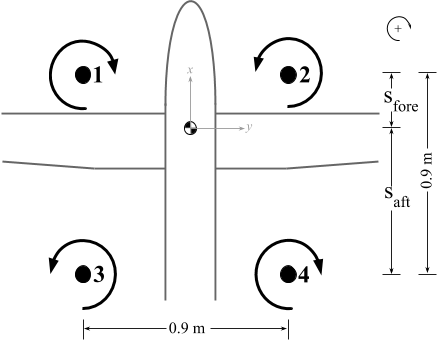
\includegraphics[width=0.6\textwidth]{StabilityandControl/Figures/Template_layout}
    \caption{Configuration with respect to the Centre of Gravity}
    \label{fig:layout}
\end{figure}

By equating the moment created by the front motors to the moment created by the aft motors around the $y$-axis the distances from the centre of gravity to the front and aft motors can be calculated. Values for S$_{fore}$ and S$_{aft}$ are presented in \autoref{tab:dist_cog_motors} below.

\begin{table}[H]
    \centering
    \caption{Table of the Distances of the Motors from the CoG}
    \begin{tabular}{lcc}
        \toprule
        \textbf{Distance} & \textbf{from min CoG [m]} & \textbf{from max CoG [m]} 
        \\ \midrule
        S$_{fore}$        & 0.229                     & 0.390
        \\ \hdashline
        S$_{aft}$         & 0.771                     & 0.610
        \\ \bottomrule
    \end{tabular}
    \label{tab:dist_cog_motors}
\end{table}

\paragraph{Pitch}
In order to perform a pitch up or down manoeuvre during vertical flight a change in moment around the $y$-axis has to be induced by the motors. As stipulated by requirement \textbf{SUB-PR-3.5} the propulsion subsystem shall be capable of providing an angular acceleration, $\alpha_{pitch}$ about the $y$-axis of 0.8 rad/s$^2$. The moment required to deliver the stipulated angular acceleration is defined as the follows:

\begin{equation}
\label{eq:requ_mome_pitc}
M_{pitch} = I_{yy} \cdot \alpha_{pitch}
\end{equation}

\nomenclature[B]{$M_{pitch}$}{Moment required for pitch manoeuvre \nomunit{N$\cdot$m}}
\nomenclature[B]{$I_{yy}$}{Moment of Inertia around the $y$-axis \nomunit{kg$\cdot$m$^2$}}

The required moment to deliver the angular pitching acceleration outlined by the requirement can then be translated into the change in thrust required ($\Delta$T) of the motor-propeller couples by dividing by the moment arms presented in \autoref{tab:dist_cog_motors}. During pitch manoeuvres it is assumed that the required moment will always be delivered by increasing the thrust of the front or aft motors-couples rather than increasing one and simultaneously decreasing the other. This is done as it is assumed that unless the UAV is in transition, the rotation of the motors will be kept to a minimum. Because of this, as the pitch motion is initiated the effective vertical force of the propellers decreases with the cosine of the angle of rotation. If the overall power was to be kept constant during pitching (by increasing either the fore or aft motors and decreasing the opposite) altitude will be lost. The loss of altitude can be mitigated by simply delivering the entire required moment with the increase of thrust of the fore \textbf{or} aft motor-propeller couples (depending on the direction of pitch required) rather than splitting the required moment over both the fore and aft motors.

\begin{figure}[H]
    \centering
    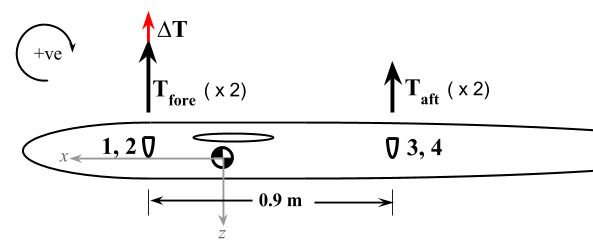
\includegraphics[width=0.6\textwidth]{StabilityandControl/Figures/Side_view_control.png}
    \caption{Side View Schematic of Pitch}
    \label{fig:schematic_side}
\end{figure}

For a pitch up manoeuvre (positive pitch) with an angular acceleration of 0.8 rad/s$^2$ the power required is calculated using equation \autoref{eq:powe_requ_pitch}. Note that this procedure is the same for a pitch down manoeuvre apart from the fact that the aft motors will be responsible for the manoeuvre as opposed to the front motors.

\begin{equation}
\label{eq:powe_requ_pitch}
P_{req} = \sqrt{\frac{(T_{fore}+\frac{\Delta T}{2})^{3}}{2 \cdot \rho \cdot A_{fore}}}
\end{equation}

Where T$_{fore}$ is the thrust of the front motor-propeller couples during hovering. The change in power required in order to deliver the required moment is therefore the difference between the power required to hover and the power required calculated above in \autoref{eq:powe_requ_pitch}.

Power can also be defined as the product of the torque delivered and the angular velocity and so by increasing the angular velocity of the propeller the power required to perform the pitch manoeuvre can be achieved. The relationship between power, torque and angular velocity is given by the following equation

\begin{equation}
\label{eq:powe_torq_angu_velo}
P = \tau \cdot \omega
\end{equation}

By increasing the voltage supplied to the motor (also increasing the power for a fixed current) the angular velocity can be increased as the angular velocity of the motor proportional to the voltage.

\paragraph{Roll}
In order to perform a pitch up or down manoeuvre during vertical flight a change in moment around the $x$-axis has to be induced by the motors. Essentially the same procedure as laid out in the above section can be employed however it is slightly more complicated given the fact that the fore and aft motors are not the same. 

\begin{figure}[H]
    \centering
    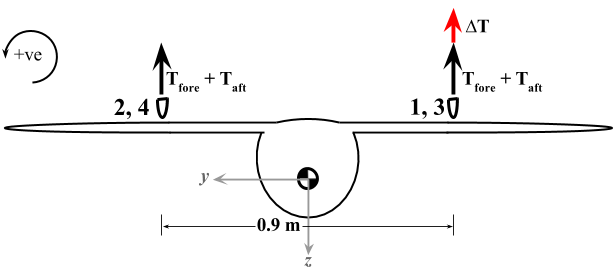
\includegraphics[width=0.6\textwidth]{StabilityandControl/Figures/Front_view_control.png}
    \caption{Front View Schematic of Roll}
    \label{fig:schematic_front}
\end{figure}

The moment required to achieve the angular acceleration stipulated by requirement \textbf{SUB-PR-3.4} is given by the equation below.

\begin{equation}
\label{eq:requ_mome_roll}
M_{roll} = I_{xx} \cdot \alpha
\end{equation}

\nomenclature[B]{$M_{roll}$}{Moment required for roll manoeuvre \nomunit{N$\cdot$m}}
\nomenclature[B]{$I_{xx}$}{Moment of Inertia around the $x$-axis \nomunit{kg$\cdot$m$^2$}}

By dividing the roll moment by the $y$-distance from the centre of gravity to the motors the combined required change in thrust ($\Delta$T) is obtained. Because the fore and aft motors are different, in order to achieve pure roll the same ratio as during hovering of thrust produced by the front propeller to the thrust produced by the aft propellers must be used. 
For a positive roll manoeuvre the power required to deliver this thrust is characterised by the following equation.

\begin{minipage}{0.48\textwidth}
    \begin{equation}
        P_{req_{1}} = \sqrt{\frac{(T_{fore}+(\frac{\Delta T}{2} \cdot \frac{T_{ratio}}{T_{ratio} + 1}))^{3}}{2 \cdot \rho \cdot A_{fore}}}
        \label{eq:powe_requ_moto_1_roll}
    \end{equation}
\end{minipage}%
\begin{minipage}{0.48\textwidth}
    \begin{equation}
        P_{req_{3}} = \sqrt{\frac{(T_{fore}+(\frac{\Delta T}{2} \cdot \frac{1}{T_{ratio} + 1}))^{3}}{2 \cdot \rho \cdot A_{fore}}}
        \label{eq:powe_requ_moto_3_roll}
    \end{equation}
\end{minipage}

Where subscripts 1 \& 3 represent motor 1 and 3 from \autoref{fig:layout} respectively as those are the motors responsible for a positive roll moment. Again, the required moment is not split across the $x$-axis in order to mitigate altitude loss because of effective vertical thrust decreasing with the cosine of angle of rotation. The change in power required for motors 1 and 3 during a positive roll manoeuvre can be achieved by increasing the angular velocity of the motors which in turn can be done by increasing the applied voltage. 

\paragraph{Yaw}
Positive or negative yaw manoeuvres during vertical flight can be performed by altering the torques of the motors. Each motor exerts a certain torque on the entire body due its rotation and this phenomenon can be exploited to perform manoeuvres. As depicted in \autoref{fig:layout} motors 1 and 4 rotate in the same direction as do motors 2 and 3 and so during yaw manoeuvres these pairs of motors will work together the provide the required moment. As stipulated by requirement \textbf{SUB-PR-3.6} the propulsion subsystem shall be capable of providing an angular acceleration, $\alpha_{yaw}$ about the $z$-axis of 0.1 rad/s$^2$. The moment required to deliver the required angular acceleration is characterised by the following equation.


\begin{equation}
\label{eq:requ_mome_yaw}
M_{yaw} = I_{zz} \cdot \alpha_{yaw}
\end{equation}

\nomenclature[B]{$M_{yaw}$}{Moment required for yaw manoeuvre \nomunit{N$\cdot$m}}
\nomenclature[B]{$I_{zz}$}{Moment of Inertia around the $z$-axis \nomunit{kg$\cdot$m$^2$}}

This moment can be achieved by altering the torque of the motors. During hovering, the torque delivered by each motor can simply be calculated by dividing the power required to hover by the nominal angular velocity of the motors during hovering. 

\begin{figure}[htb]
    \centering
    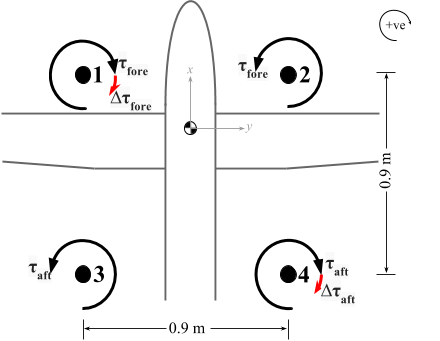
\includegraphics[width=0.6\textwidth]{StabilityandControl/Figures/Top_view_control.png}
    \caption{Top View Schematic of Roll}
    \label{fig:schematic_top}
\end{figure}

For a positive yaw manoeuvre the change in torque ($\Delta \tau$) required is split up over motor 1 and 4 (from \autoref{fig:layout}). This torque is split up according to the ratio of torque of motor 1 to torque of motor 4 (please note that for a negative yaw manoeuvre the same procedure is applied except the opposite motor pairs will be increasing or decreasing power respectively). The change in power ($\Delta$P) of the motors delivering the manoeuvre (i.e. motors 1 and 4) as a result of the increase in torque required can be calculated by multiplying the torque required of each motor with their respective angualar velocities as shown in Equations \ref{eq:powe_requ_moto_1_yaw} \& \ref{eq:powe_requ_moto_4_yaw}. \newline

\begin{minipage}{0.48\textwidth}
    \begin{equation}
    \label{eq:powe_requ_moto_1_yaw}
    \Delta P = \Delta \tau_1 \cdot \omega_1
    \end{equation}  
\end{minipage}%
\begin{minipage}{0.48\textwidth}
    \begin{equation}
    \label{eq:powe_requ_moto_4_yaw}
    \Delta P = \Delta \tau_4 \cdot \omega_4
    \end{equation}
\end{minipage}
\newline

In order to maintain altitude this change in power (increase) must be countered by a decrease in power from the other two motors, namely motors 2 and 3. The increase in power required of motor 1 (from \autoref{eq:powe_requ_moto_1_yaw}) needs to be subtracted from the power required of motor 2 to hover and likewise the increase in power required of motor 4 (from \autoref{eq:powe_requ_moto_4_yaw}) needs to be subtracted from the power required of motor 3 to hover.

In order to ensure that the required torque is delivered, the positive change in power required of motors 1 and 4 should be achieved by increasing the current delivered to the said motors as torque is proportional to current. The decrease in power of the remaining two motors can simply be achieved by decreasing the respective angular velocities by lowering the applied voltage.

\paragraph{Results}
The following tables breaks down the required power to perform the three outlined manoeuvres.


\begin{table}[H]
\centering
\caption{Table of Power Required for Motors 1 \& 2}
\label{tab:powe_requ_moto_1_2}
\begin{tabular}{lll|cc|cc|}
\cline{4-7}
                           &                            &                                  & \multicolumn{2}{c|}{\textbf{Motor 1}}    & \multicolumn{2}{c|}{\textbf{Motor 2}}    \\ \cline{4-7} 
                           &                            &                                  & \textbf{c.g.$_{min}$}    & \textbf{c.g.$_{max}$}    & \textbf{c.g.$_{min}$}    & \textbf{c.g.$_{max}$}    \\ \hline
\multicolumn{1}{|l}{\textbf{Hover}} & \multicolumn{1}{l|}{}      & P$_{req}$ {[}W{]}                & 2423.89        & 1553.15        & 2423.89        & 1553.15        \\ \hline
\multicolumn{1}{|l}{\textbf{Pitch}} & \multicolumn{1}{l|}{+ve}   & P$_{req}$ {[}W{]}                & 2519.14        & 1599.12        & 2519.14        & 1599.12        \\ \hdashline
\multicolumn{1}{|l}{}      & \multicolumn{1}{l|}{$-$ve} & P$_{req}$ {[}W{]}                & 2423.89        & 1553.15        & 2423.89        & 1553.15        \\ \hline
\multicolumn{1}{|l}{\textbf{Roll}}  & \multicolumn{1}{l|}{+ve}   & P$_{req}$ {[}W{]}                & 2472.59        & 1584.35        & 2423.89        & 1553.15        \\ \hdashline
\multicolumn{1}{|l}{}      & \multicolumn{1}{l|}{$-$ve} & P$_{req}$ {[}W{]}                & 2423.89        & 1553.15        & 2472.59        & 1584.35        \\ \hline
\multicolumn{1}{|l}{\textbf{Yaw}}   & \multicolumn{1}{l|}{+ve}   & P$_{req}$ {[}W{]}                       & 2774.47        & 1806.77        & 2073.30        & 1299.52        \\ \hdashline
\multicolumn{1}{|l}{}      & \multicolumn{1}{l|}{}      & ($\Delta \tau$, $\Delta \omega$) & (0.74 , 0.0)   & (0.54 , 0.0)   & (0.0 , -68.16) & (0.0 , -76.95) \\ \hdashline
\multicolumn{1}{|l}{}      & \multicolumn{1}{l|}{$-$ve} & P$_{req}$ {[}W{]}                       & 2073.30        & 1299.52        & 2774.47        & 1806.77        \\ \hdashline
\multicolumn{1}{|l}{}      & \multicolumn{1}{l|}{}      & ($\Delta \tau$, $\Delta \omega$) & (0.0 , -68.16) & (0.0 , -76.95) & (-0.74 , 0.0)  & (-0.54 , 0.0)  \\ \hline
\end{tabular}
\end{table}

\begin{table}[H]
\centering
\caption{Table of Power Required for Motors 3 \& 4}
\label{tab:powe_requ_moto_3_4}
\begin{tabular}{lll|cc|cc|}
\cline{4-7}
                           &                            &                                  & \multicolumn{2}{c|}{\textbf{Motor 3}}      & \multicolumn{2}{c|}{\textbf{Motor 4}}      \\ \cline{4-7} 
                           &                            &                                  & \textbf{c.g.$_{min}$}    &\textbf{ c.g.$_{max}$}     & \textbf{c.g.$_{min}$}     & \textbf{c.g.$_{max}$}     \\ \hline
\multicolumn{1}{|l}{\textbf{Hover}} & \multicolumn{1}{l|}{}      & P$_{req}$ {[}W{]}                & 661.58          & 1575.57         & 661.58          & 1575.57         \\ \hline
\multicolumn{1}{|l}{\textbf{Pitch}} & \multicolumn{1}{l|}{+ve}   & P$_{req}$ {[}W{]}                & 661.58          & 1575.57         & 661.58          & 1575.57         \\ \hdashline
\multicolumn{1}{|l}{}      & \multicolumn{1}{l|}{$-$ve} & P$_{req}$ {[}W{]}                & 693.91          & 1633.53         & 693.91          & 1633.53         \\ \hline
\multicolumn{1}{|l}{\textbf{Roll}}  & \multicolumn{1}{l|}{+ve}   & P$_{req}$ {[}W{]}                & 674.88          & 1607.22         & 661.58          & 1575.57         \\ \hdashline
\multicolumn{1}{|l}{}      & \multicolumn{1}{l|}{$-$ve} & P$_{req}$ {[}W{]}                & 661.58          & 1575.57         & 674.88          & 1607.22         \\ \hline
\multicolumn{1}{|l}{\textbf{Yaw}}   & \multicolumn{1}{l|}{+ve}   & P$_{req}$ {[}W{]}                       & 565.89          & 1318.28         & 757.27          & 1832.86         \\ \hdashline
\multicolumn{1}{|l}{}      & \multicolumn{1}{l|}{}      & ($\Delta \tau$, $\Delta \omega$) & (0.0 , -113.60) & (0.0 , -128.25) & (0.12 , 0.0)    & (0.33 , 0.0)    \\ \hdashline
\multicolumn{1}{|l}{}      & \multicolumn{1}{l|}{$-$ve} & P$_{req}$ {[}W{]}                       & 757.27          & 1832.86         & 565.89          & 1318.28         \\ \hdashline
\multicolumn{1}{|l}{}      & \multicolumn{1}{l|}{}      & ($\Delta \tau$, $\Delta \omega$) & (-0.12 , 0.0)   & (-0.33 , 0.0)   & (0.0 , -113.60) & (0.0 , -128.25) \\ \hline
\end{tabular}
\end{table}


\subsection{Transition}
The transition phase is defined by two sequences, namely the transition from vertical flight to horizontal flight and the transition from horizontal flight to vertical flight. Each sequence requires a different set of steps in order to be carried out. Only steps required to transition from vertical flight to horizontal flight will be outlined however it is important to note that the steps required to transition from horizontal back to vertical flight are essentially the inverse. %A brief description of the transition from horizontal to vertical flight will be presented.

%\paragraph{Vertical to Horizontal Flight}
Hovering is the least power intensive sector of the vertical flight phase apart from decent and therefore it is assumed that transition commences from rest (zero velocity and by definition constant altitude). During hovering, moment equilibrium holds to maintain attitude and therefore in order to ensure that both altitude and attitude are conserved during transition, both the moment equilibrium about the centre of gravity as well as vertical force equilibrium need to hold.

In order to perform the transition, horizontal velocity needs to be introduced. This is done by rotating the aft motors counterclockwise from there hovering position (pointing in the positive $z$-direction, thrust vector pointing upward). Simultaneously the thrust level of the aft motors must be increased to counteract the vertical thrust decrease because of the rotation.

As horizontal velocity increases, lift generated by the wing increases linearly with the square of velocity (i.e. $L \propto V^2$). This means that by subtracting the lift as a function of velocity (which is therefore a function of time) the total vertical thrust required during transition will decrease. 

\autoref{fig:tran_vert_to_hori} graph of angle of rotation of the aft motor versus the horizontal velocity illustrates the transition. It is apparent from the graph that for the most aft centre of gravity location there is no problem attaining the stall velocity of 20 m/s before the aft motors have rotated a complete 90 $^{\circ}$. For the most forward centre of gravity location, this is not the case however, once the aft motor has completely rotated additional thrust is required to gather enough velocity to generated sufficient lift from the wing. This is not a problem however as the front motor, being substantially closer to the most forward centre of gravity location, can provide enough lift to maintain altitude. Whatever moment around the centre of gravity created by the front motors can now be countered with the elevator as, with a velocity of approximately 15 m/s the elevator is sufficiently effected to deliver small control moments. 

\begin{figure}[H]
    \centering
    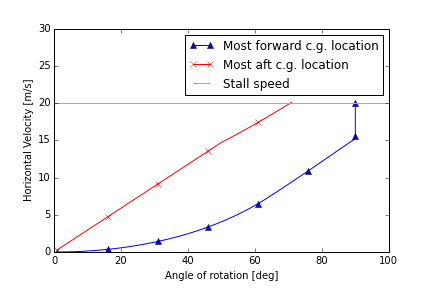
\includegraphics[width=0.6\textwidth]{StabilityandControl/Figures/transition.png}
    \caption{Graph of Angle of Rotation vs. Horizontal Velocity}
    \label{fig:tran_vert_to_hori}
\end{figure}

\section{Verification \& Validation}
\label{sec:veri_vali_snc}
In this section the verification and validation of the stability and control analysis and design is performed.

\paragraph{Tail Configuration}
The T-tail configuration choice can be validated by confirming that the downwash caused by the wing calculated using xflr5 is in the order of magnitude of 0.001. Since this was one of the main reasons the T-tail was chosen, it can be considered validated.

The incidence angle of the horizontal tailplane was checked by inspecting if the angle has a realistic value. Angles between -3 and 3 degrees are typically used \cite[67]{raymer}. Hence, the design value of 2.6 degrees lies within realistic boundaries.

\paragraph{Longitudinal Stability \& Control}
The c.g. position as a function of the leading edge calculated in the c.g. plot can be verified by calculating the actual c.g. position of the final CATIA model for the actual leading edge position and comparing it to the point on the curve. Due to time constraints, this was not possible but it can be considered as a future recommendation. The c.g. position is now verified by making hand calculations for the minimum and maximum c.g. range for a certain leading edge position and comparing it to the value in the python code. Another way the c.g. plot was verified was to check if special inputs (e.g. all masses zero, all arms zero, all arms in the middle) also gave the required, known output (e.g. error because of dividing by zero, c.g. is zero, c.g. is in the middle). Finally, a sanity check was performed on the final c.g. range. For example: checking whether the c.g. lies inside the fuselage.

The scissor plot can be validated by checking if all the assumptions used in the model for the stability and control curve are valid. In \autoref{sec:assu_snc}, all assumptions used are explained and the effects and deviations from reality are mentioned. As can be seen, the assumptions needed for the control and stability curve are only deviating slightly. The calculations are verified by checking if the input coefficients all have the correct sign and magnitude. For instance, the minimum tail lift coefficient should not exceed minus one, the lift slope coefficient should be positive and have a magnitude of one. The results of the scissor plot can be verified by performing a sanity check. Attention can be paid to the slope and the shift of the curves. For example, the neutral point should lie behind the leading edge, the slope of the control curve should be negative and the slope of the stability curve should be positive.

\paragraph{Lateral/Directional Stability \& Control}
The method used to size the vertical tailplane was validated by comparing the calculated surface area with that of the surface area estimated through the statistical method outlined in literature \cite[112]{raymer}. The method based on statistics makes use of typical vertical tail volume coefficients (c$_{vt}$) from which the surface area can by calculated as follows:

\begin{equation}
\label{eq:vert_tail_coef}
S_{vertical} = \frac{c_{vt} \cdot b_{w} \cdot S}{l_{v}}
\end{equation}

It is very difficult to find typical vertical tailplane volume coefficients for UAVs however using a typical value for light aircraft, a surface area in the same order of magnitude is obtained (S$_{vertical}$ of 0.04 m$^{2}$).

\paragraph{Control Surfaces}
In order to check the control surface results, the moment generated by the control surface was calculated by hand and checked with the required moment it is supposed to generate. Also, the code was checked by putting different values for deflection angles (e.g. delta = 0 deg, delta = 30 deg) in the code and verifying if the outputs are reasonable.

The maximum hinge moment produced by the control surfaces was verified by doing the calculation by hand for the maximum deflection angle and checking whether the values comply.

\paragraph{Vertical Flight Manoeuvres}
The required power splits were calculated using a python script. This script was validated by calculating the inverse, beginning with the outputs and seeing whether the inputs were obtained as results. The inputs of the main python script were also validated with had calculations to ensure that the script was executed using valid inputs. 

Another way the the script was validated was by setting the angular accelerations for pitch, roll and yaw ($\alpha{pitch}$, $\alpha{roll}$ \& $\alpha{yaw}$) to zero. This was done to ensure that the output of the code, given this condition, was simply the power split calculated for hovering.


%recommendations: investigate dynamic stability